Exploring variants to the baseline solution serves multiple purposes.  First, several available methods and data sets were not included in the baseline solution, for various reasons---primarily because of maturity of analysis or questions about uncertainty estimates. These data can still be used to highlight potential issues with the baseline solution, or point toward future research directions. In some cases, additional observations may eventually justify including these methods in the baseline. Second, it is informative to assess what happens to both the value and uncertainty in the Hubble constant when different categories of data are included or excluded in the solution. Third, some methods\hbox{---}e.g., SNe~Ia\hbox{---}can be included in several different ways; different filters, different light curve analysis, or different redshift selections. Finally, it is useful to consider a solution that includes all available, independent data and methods to assess the potential precision achievable with existing data once the remaining analysis issues are resolved. We stress that our process determined the baseline analysis as the primary solution \textit{priori to} obtaining any results on \Hcst{}. 
Variants in these categories are defined in Section~\ref{sec:variant_description}, and the results discussed in Section~\ref{sec:variant_results}.

Separately, we also consider two additional sets of consistency checks presented in Sect.\,\ref{sec:consistency_both}. One builds fully independent, ``orthogonal'' paths capable of determining \Hcst{} to verify that no single path/method dominates the \DN{}, cf. Section~\ref{sec:orthogonal_paths}.
The other employs a variety of different, albeit not independent, paths through the data to verify that their statistical properties are consistent with expectations, cf.~Section~\ref{sec:consistency_checks}. These checks serve to demonstrate the statistical consistency of the baseline solution with all possible configurations. Replications of results presented in the literature provide additional consistency checks of our methodology and are presented in Appendix~\ref{sec:comparisons}.


Some general considerations pertain to all these analyses and their interpretation. First, the baseline and variants were defined and classified {\it before} considering the resulting values of {\Hcst}. Very minor changes were introduced afterwards if required by updated data availability, albeit without changing the definition of the baseline.  
Second, most ``variants'' should not be regarded as alternative, equally valid solutions. Rather, their role is to illustrate the statistical properties of the data, identify potential problems, and/or reinforce their validity. This is especially true when considering the consistency checks, which are designed specifically so that each path uses only a small fraction of the available data, and thus has by construction a large nominal uncertainty, which is \textit{in no way} representative of the uncertainty in {\Hcst}. Third, the results of all variants are highly correlated because they share large portions of data. An exception are the orthogonal paths in Section~\ref{sec:orthogonal_paths}, which serve as consistency checks. Hence, the scatter between variants is expected to be much smaller than their error estimates. 

\subsection {Description of variants}\label{sec:variant_description}

The following is a short description of the main variants included in Table~\ref{tab:variants}. Specific sources of data products are provided in the text and in Appendix~\ref{sec:data_appendix}.

\begin{itemize}
\item[]\textbf{Baseline}
    \item[V00] Baseline: includes all measurements of SNe~Ia host distances using either Cepheids or TRGB, with the Milky Way via \gaia, the LMC, and NGC$\,$4258 as anchors, as well as SBF calibrated via TRGB and megamasers in the Hubble flow.   Note that TRGB distances are only anchored to NGC$\,$4258, since TRGB calibrations from the Milky Way and LMC do not meet our data requirements (notably photometric homogeneity across anchors and hosts in HST/JWST passbands).  Cepheids use all three anchors.  
    \smallskip\item[]\textbf{Add-one-in variants}
    \item[V01] Baseline + JAGB: includes all baseline methods, plus measurements of SNe~Ia hosts using the JAGB method, calibrated to NGC$\,$4258.
    \item[V02] Baseline + Miras: includes all baseline methods, plus measurements of SNe~Ia hosts using  Mira variables, calibrated to NGC$\,$4258.
    \item[V03] Baseline + Fundamental Plane: includes all baseline methods, plus distances to elliptical galaxies using the Fundamental Plane as measured by DESI, and calibrated to the distance of the Coma cluster measured with SBF and SNe~Ia.
    \item[V04] Baseline + empirically calibrated SNe II: includes all baseline methods and adds SNe~II (standard candle method) both as calibrators and in the Hubble Flow.  SNe~II host distances are determined via the distance network.
    \item[V05] Baseline + SNe~II with Expanding Photosphere Method: includes all baseline methods, plus SNe~II distances measured by the (astrophysical model-dependent) Expanding Photosphere Method.  Excludes a handful of supernovae that are too nearby to have significant weight on the determination of $ H_0 $.
    \item[V06] Baseline + Tully-Fisher: includes all baseline methods and adds calibrators for the Tully-Fisher relation and Tully-Fisher galaxies in the Hubble flow. The calibrators are treated in the same way as SNe Ia hosts, and their individual distances are determined from all available measurements.
    \item[V07] Baseline + SMC as anchor: includes all baseline methods and includes the SMC as an additional anchor for Cepheids.
    \smallskip\item[]\textbf{Leave-one-out variants}
    \item[V08] Baseline without Cepheids: excludes all Cepheid measurements from the distance network.  As a consequence, it only uses NGC$\,$4258 as anchor, since the Milky Way and LMC are currently only used via Cepheids. It furthermore excludes some SNe Ia for which TRGB measurements are not available.
    \item[V09] Baseline without TRGB: excludes all TRGB-based measurements.  As a consequence, it excludes some SNe Ia for which Cepheid measurements are not available, and the SBF method, which in this version it is only calibrated via TRGB.  A future version could include other primary distance indicators to calibrate the SBF method.
    \item[V10] Baseline without parallaxes: excludes parallaxes measured by {\it Gaia} and {HST}. As a consequence, the MW is removed as an anchor.
    \item[V11] Baseline without DEB distances to the LMC: removes the LMC as an anchor.  Note that the SMC is not included in the baseline.
    \item[V12] Baseline without NGC$\,$4258: this excludes all measurements based on NGC 4258 as anchor. As a consequence, all TRGB measurements are removed, since they are exclusively calibrated via NGC$\,$4258. As in V09, this also results in the exclusion of a number of SNe Ia for which no Cepheid measurements are available, as well as the SBF method.
    \item[V13]  Baseline without SNe~Ia: excludes all SNe~Ia, both as calibrators and as Hubble Flow objects.
    \item[V14]  Baseline without SBF: excludes all SBF-measured galaxies in the Hubble Flow.
    \item[V15]  Baseline without masers in the Hubble flow: retains the maser distance to NGC$\,$4258, but excludes other megamaser measurements. 
    \smallskip\item[]\textbf{Instrument-suspicious variants}
    \item[V16]  Exclude HST data: excludes {\it all} HST data from the baseline.  Since JWST anchor measurements are only available for NGC$\,$4258, this version also excludes the Milky Way and the LMC as anchors. 
    \item[V17]  Exclude JWST data: removes all JWST observations from the baseline.
    \item[V18]  Exclude SN~1994D and earlier: excludes 7 SNe~Ia calibrators that do not have modern data, namely SN 1980N, 1981B, 1981D, 1989B, 1990N, 1992A, and 1994D.
    \smallskip\item[]\textbf{Custom baselines}
    \item[V08B] Modified baseline for the no-Cepheid variant V08.  This is identical to the baseline, except that SNe~Ia for which we only have Cepheid distance estimates have been removed, leaving 35 SNe Ia calibrators.  Comparing V08 and V08B allows a direct estimate of the impact of removing Cepheids from the distance network, without the effect of changing the subset of SNe~Ia calibrators.
    \item[V09B] Modified baseline for the no-TRGB variant V09. This is identical to the baseline, except that SNe~Ia for which we only have TRGB distance estimates have been removed, leaving 42 SNe Ia calibrators. Comparing V09 and V09B allows a direct estimate of the impact of removing TRGB from the distance network, without the effect of changing the subset of SNe~Ia calibrators. However, this custom baseline includes SBF, which are excluded from V09 because they are calibrated using TRGB distances; therefore the difference between V09 and V09B is due to both the TRGB contribution to SN calibrator distances and to the omission of SBF.
    \item[V12B] Modified baseline for the no-NGC 4258 variant V12.  This is identical to the baseline, except that SNe~Ia for which we only have  distance estimates based on NGC 4258 have been removed, leaving 42 SNe Ia calibrators.  This variant allows a direct estimate of the impact of removing NGC 4258 from the distance network, without the effect of changing the subset of SNe~Ia calibrators.  Unlike V09B, this custom baseline also excludes SBF measurements;
    therefore the difference between V12 and V12B is only in the contribution of NGC 4258 to the distances to SNe Ia calibrators.  
    \item[V16B] Modified baseline for the no-HST variant V16. This is identical to the baseline, except that SNe~Ia for which we only have HST-based distance estimates have been removed, leaving 24 SNe Ia calibrators. Comparing V16 and V16B allows a direct estimate of the impact of removing HST measurements from the distance network, without the effect of changing the subset of SNe~Ia calibrators.
    \smallskip\item[]\textbf{Hypothesis-driven variants} 
    \item[V19] Modified baseline in the CMB frame: removes the peculiar velocity corrections for SNe~Ia, SBF, and megamasers in the Hubble flow.
    \item[V20] Modified baseline that limits Hubble flow SNe~Ia to $ 0.023 \leq z \leq 0.06 $.
    \item[V21] Modified baseline, with SNeIa in the Hubble flow limited to $ 0.03 \leq z \leq 0.1 $.
    \item[V22] Modified baseline, with SNeIa restricted to the CSP sample fit using SNooPy v2.7 for both calibrators and tracers. 
    \item[V23] Modified baseline with SNe~Ia measurements fitted using BayesSN for both calibrators and Hubble flow objects.
    \item[V24] Modified baseline, wherein SNe\,Ia light curves were fitted using the SALT V3 fitter instead of SALT V2.4 (as in Pantheon+)
    \item[V25] Modified baseline that exclusively uses H-band NIR measurements for both calibrators and Hubble flow SNe~Ia.
    \item[V26] Modified baseline that exclusively uses J-band NIR measurements for both calibrators and Hubble flow SNe~Ia.
    \item[V27] Modified baseline that ignores off-diagonal covariance terms for Hubble flow SNe~Ia.
    \item[V28] Modified baseline without metallicity corrections for Cepheid PL relation
    \smallskip\item[]\textbf{Include everything}
    \item[V99] ``Everything'': All data included in any variant, without repeating Hubble Flow objects; SNe~Ia exclusively from Pantheon+.
   \item[V99a] ``Everything but Tully-Fisher'': as V99, but excludes the Tully-Fisher method, which contributes to the total $ \chi^2 $ beyond expectations, and has high $ \chi^2 $ in the Hubble Flow.
\end{itemize}

\input Tables/vartable.tex

\begin{figure}
    \centering
    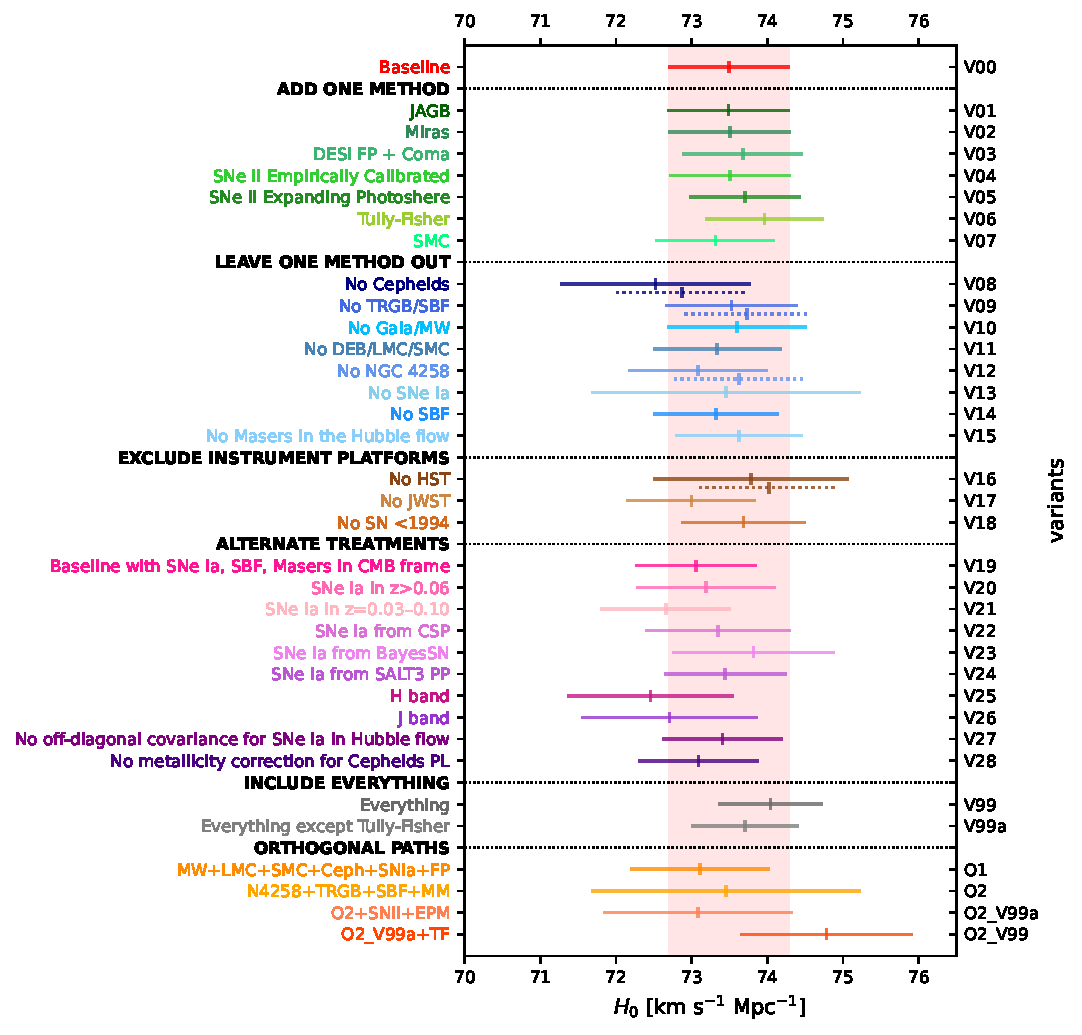
\includegraphics[width=\linewidth]{Figures/H0_whisker_solid.pdf}
    \caption{Baseline and variants results from Table~\ref{tab:variants}. For some variants, a labeled change has a secondary consequence (i.e., removing the identified primary distance indicator also results in the loss of calibration to some SN Ia).  In these cases a dashed line immediately below such variants provides a custom baseline--i.e., the same SNe are removed before the removal of the primary indicator--is shown to provide a custom reference of impact for that variant; see text for details.
    }
    \label{fig:whisker}
\end{figure}

\subsection{Overview of results based on variants} \label{sec:variant_results}

The results of the baseline and all variants are illustrated in Figure\ref{fig:whisker} and reported in Table~\ref{tab:variants}. All variants yield results consistent with the baseline, typically varying only slightly from the baseline result; the dispersion of central values is $0.400$\,\Hunit, or $50\%$ of the baseline's $1\sigma$ uncertainty. Since the baseline and its variants are highly correlated due to shared datasets and methodologies, a scatter significantly below $1\sigma$ is expected. The absence of outliers among the variants demonstrates that the results are not driven in any particular direction by any one dataset or methodology, or any of the hypothetical systematics explored. For example, variants V08, V10, and V13 demonstrate that the central value of {\Hcst} is not dominated by Cepheids (V08), parallaxes mainly from {\it Gaia} (V10), or SNe~Ia (V13).  
Figure~\ref{fig:whisker} also readily identifies differences in constraining power brought by various methods: the largest increases in the error on \Hcst{} are seen in V08 (no Cepheids), V13 (no SNe\,Ia), and V16 (no HST). This underlines the crucial precision provided by Cepheids, SNe\,Ia, and {HST} observations, whereas the insensitivity of the central value on \Hcst{} demonstrates that neither dominate the result.
The exploration of such variants establishes robustness of the baseline result and demonstrates that the {\DN} is enhanced by the joint consideration of complementary methodologies. It further underlines that the different methodologies reinforce and strengthen each other, resulting in improved accuracy thanks to the DN approach.  

\subsubsection {Adding one class at a time}

Variants V01 to V07 each add one category of objects or methodology to the baseline solution; these include JAGB, Miras, the Fundamental Plane of elliptical galaxies, empirically and astrophysically calibrated SNe~II, Tully-Fisher, and the SMC as an additional anchor.  For all cases except the Tully-Fisher relation, the impact on the solution is negligible, with the central value of $ H_0 $ changing by 0.2 {\Hunit} or less ($25\%$ of the $1\sigma$ uncertainty), and the uncertainty remaining constant or decreasing slightly.  Including astrophysically calibrated SNe~II (V05) leads to the most significant improvement to the uncertainty, by $8.5\%$ to $ \Herrorepm \Hunit $; however, this method being relatively new, its systematic uncertainties are not yet fully quantified \citep{2025AA...702A..41V}.  

Including the Tully-Fisher relation raises $ H_0 $ by almost 0.5 {\Hunit} ($\sim 60\%$ of the baseline error), and yields a reduced $ \chi^2 $ significantly larger than unity (\redchisqtf). The increase in $ H_0 $ is consistent with the results of the recalibration of the Tully-Fisher relation by \cite{2024arXiv241208449S}.  Inspection of the residuals shows that the anomalous value of $ \chi^2 $ is caused by the dispersion in predicted magnitude for Tully-Fisher calibrators, whose empirical scatter significantly exceeds the assumed intrinsic dispersion, particularly at the bright end. Uncertainties in host distances are subdominant and unlikely to play a role in this comparison. We conclude that the internal dispersion currently assumed for the Tully-Fisher relation is likely underestimated, and recommend avoiding the inclusion of Tully-Fisher results until its intrinsic dispersion can be reevaluated.

 \subsubsection {Leave-one-out variants\label{sec:leave-one-out}}

Variants V08-V18 each remove one class of measurements or a subset of data from the solution.  Most variants do not change the central value of {\Hcst} much, with the exception of V08 (no Cepheids), which drops it by almost 1 {\Hunit} to {\Hvaluenoceph} {\Hunit}, and V12 (no NGC 4258), which decreases it to {\Hvaluenoftfe} {\Hunit}. 
Comparing V08 and the corresponding custom baseline (V08B) clearly identifies that the shift in the no-Cepheids variant (V08) is driven by the implicit exclusion of 20 calibrator SNe\,Ia rather than by the Cepheids themselves. Analogous effects on \Hcst{} induced by subsampling SNe\,Ia calibrators have been extensively discussed in \citet{2024ApJ...977..120R}. Accounting for this effect leaves a difference of merely $0.352$\,\Hunit\ ($44\%$ of the baseline error) due to excluding Cepheids.

Some variants yield significantly increased uncertainties on \Hcst{}. Excluding Cepheids (V08) increases the uncertainty from {\Herrorbase} to {\Herrornoceph} {\Hunit}, and comparison with the uncertainty of the custom baseline V08B (\Herrorcustbasenoceph) reveals that this increase is truly driven by the exclusion of Cepheids rather than the implicitly removed 20 SNe\,Ia calibrators. 
More modest increases occur for the variants without NGC$\,$4258 as anchor, or when TRGB measurements are excluded. This is simply a reflection of the reduced constraining power caused by the exclusion of a broad class of measurements. Excluding either the Milky Way or the LMC as anchors has less impact, as each exclusion leaves two anchors for Cepheids, and does not affect the TRGB, which is only calibrated via NGC$\,$4258. The most dramatic impact is associated with the exclusion of all SNe~Ia; this increases the uncertainty to {\Herrornosnia} {\Hunit}, more than a factor of 2 above the baseline, illustrating the strong constraining power of SNe~Ia, which remain the most powerful way to measure the local value of the Hubble constant. 
When SNe Ia are excluded from the baseline, the primary constraint on {\Hcst} is based on the SBF measurement. Even in this case, the central value of {\Hcst} is changed only little, although one naturally finds a much larger uncertainty. As an illustration, the solution including all other available data but excluding SNe~Ia in the Hubble flow---formally not a variant, since it does not satisfy the criteria established during the Workshop---yields $ \Hvaluehfnosnia \pm \Herrorhfnosnia \, \Hunit $; despite the higher uncertainty, this value is still $\Hsigmahfnosnia \, \sigma $ away from the CMB value in flat $\Lambda$CDM.

The two variants V16 and V17 explore the impact of excluding all calibrator  data from either HST or JWST, testing potential broad systematics, such as calibration errors, that affect either facility. Note that all primary distance indicators as included used space-based data from at least one of the two facilities.
Excluding HST also implies excluding the Milky Way and the LMC as anchors, since we do not yet have a calibration for Cepheids in those systems based on JWST data.  The solutions with either no HST or no JWST data are not fully disjoint since they share a common anchor, NGC 4258, and many of the Hubble Flow tracers, and since the set of calibrators overlap, carrying with them any intrinsic variance in their properties.  However, many of the sources of uncertainty in distance estimates are different and independent. The resulting {\Hcst} values bracket the baseline, as could be expected, with a difference in line with their respective uncertainties: without HST, $ \Hvaluenohst \pm \Herrornohst \, \Hunit $; and without JWST, $ \Hvaluenojwst \pm \Herrornojwst \, \Hunit $.  Not surprisingly, the uncertainty in the result increases more if HST is excluded, since HST results use three anchors (only NGC 4258 is available for JWST) and more HST observations are available, yet both subsets remain close to the baseline with a difference below $ 1 \, \Hunit $. The fact that the inclusion of JWST observations favors a higher value of \Hcst{} corroborates the conclusion based on host-to-host distance comparisons by \citet{2024ApJ...977..120R} that \Hcst{} measurements based purely on HST \citep{2022ApJ...934L...7R} are not biased high by the limited spatial resolution of WFC3/IR (crowding).

\subsubsection {Alternate treatments\label{sec:alternative_medicine}}

Variants V19-V26 show what happens if subsets of data are either excluded or treated differently. For variants V19-V22, we modify the handling of peculiar velocities or redshift selection. In variant V19, we assume that the observed velocities directly represent cosmological redshifts, i.e., we set all peculiar velocity corrections, which are by default derived with the 2M++ model \citep{2015MNRAS.450..317C}, to zero.  The value of {\Hcst} decreases slightly, to $ {\Hvalueusecmb} \pm {\Herrorusecmb} \, \Hunit $, with no meaningful change in the accuracy.
Similarly, restricting the redshift range, either by removing the high redshift end (V20, $ z > 0.06 $) or the low-redshift end (V21, $ 0.3 < z < 1 $), changes the value of {\Hcst} by up to 0.8\,{\Hunit}; the impact on the accuracy is modest.

Variants V22-V27 are noteworthy because they explore different treatments of SNe\,Ia, which drive overall precision (cf. Sect.\,\ref{sec:leave-one-out}). 
Variants V22 and V23 consider different light curve fitters (consistently for both calibrators and tracers), namely SNooPy v2.7 in V22 and BayesSN in V23. Both variants yield slightly higher \Hcst{} values with slightly larger nominal uncertainties. The BayesSN variant V23 furthermore yields a higher reduced $ \chi^2 $. Further detail and comparisons with published articles is provided in App.\,\ref{app:sec:SNIa_literature}, specifically concerning SNooPy in App.\,\ref{app:snoopy}.

Variants V25 and V26 rely exclusively on NIR measurements for SNe~Ia \citep{2023AA...679A..95G}, in the $ H $ and $ J $ band respectively. These also yield slightly lower, yet consistent \Hcst{} results with slightly larger uncertainties due to the smaller number of calibrators and Hubble flow tracers.  Note that we did \textit{not} use SNe~Ia measurements from multiple sources (e.g., Pantheon+ and NIR) simultaneously in any solution; doing so would lead to unreliable, likely incorrect results.  First, the calibration of SN measurements in different samples are inconsistent, as they are based on different filters, fitting processes, and conventions.  More importantly, different measurements of the same SN would share to a large extent the astrophysical variance of the source; therefore we expect such measurements to be significantly correlated in their deviation from the mean, to an extent that; to the best of our knowlegde, has not been sufficiently quantified.  Since the SNe~Ia samples overlap significantly, multiple measurements cannot be included in the same solution in a statistically satisfactory way.  To avoid such issues, we take care not to include multiple measurements of the same SNe~Ia---whether as local calibrators or as Hubble flow objects---in the same solution. Unless otherwise stated, all solutions exclusively consider measurements collected in the Pantheon+ system \citep{2022ApJ...938..113S}.

Another treatment option concerns the covariance between different SNe~Ia in the Hubble flow. Several collections of measurements provide covariances between different objects; these can be due to the effect of standardization parameters, or the survey from which data have been obtained. By default, we include such covariances where available. However, Variant V27 deliberately ignores these covariances and assumes (incorrectly) the stated uncertainties to be independent in order to assess the impact that the SNe\,Ia covariances have on the final result. This results in a miniscule decrease in {\Hcst}, by less than 0.1\,{\Hunit}, and analogously miniscule decrease in the nominal uncertainty. We conclude that covariances between SNe~Ia measurements in the Hubble flow currently have a negligible impact on \Hcst. 

\subsubsection {``Everything'' solution\label{sec:everything_bagel}}

It is naturally interesting to consider the result of including all available methods into the \DN{}. To this end, we constructed variant V99 by including all available measurements.
As noted above, multiple measurements of SNe~Ia cannot be combined in a statistically satisfactory way, so that V99 exclusively considered Pantheon+ SNeIa. V99 also incorporates methods with as yet insufficiently well understood systematics, such as SN~II with EPM and the Tully-Fisher relation. 
These results are provided here for completeness, and we recommend that they \textit{not} be used for further analysis.  The resulting value is $ \Hvalueeverything \pm \Herroreverything \, \Hunit $, which lies $ \Hsigmaeverything \, \sigma $ from the Planck+$\Lambda$CDM solution.  We recognize that this solution may not be fully reliable, as indicated by the relatively large value of reduced $ \chi^2 $, namely $\redchisqeverything $ per degree of freedom; indeed, this solution deviates from the baseline more than several others, primarily because of the TF contribution.  Since the TF relation contributes the most to the excess $\chi^2 $, we also include variant V99a, which is identical to V99 except for the exclusion of TF calibrators and tracers.  This variant results in $ \Hcst = \Hvalueeverythingnotf \pm \Herroreverythingnotf \Hunit $, very close to the baseline with a 12\% smaller uncertainty (and sub-percent precision on \Hcst), has a reasonable reduced $ \chi^2 $ of {\redchisqeverythingnotf}, and lies $ \Hsigmaeverythingnotf \, \sigma $ from the Plank+$\Lambda$CDM solution. 

The everything solution is useful to understanding how elements in the baseline solution compare to the elements not included therein, as well as any covariances among them. Three figures illustrate these points. Figure\,\ref{fig:everything_residuals} shows the fit residuals of host and calibrator distances for V99 in analogy with Fig.\,\ref{fig:baseline_residuals} for the baseline. Figure\,\ref{fig:everything_hf} illustrates the corresponding Hubble flow residuals for V99. A corner plot illustrating covariance among the main global fit parameters of the \DN{} for V99 is shown in Fig.\,\ref{fig:everything_corner}. 

\begin{figure*}
    \centering
    \includegraphics[width=0.9\linewidth]{Figures/ISSI-H0-Workshop-DistanceNetwork-all-batlowKS.pdf}
    \caption{Residuals for host and calibrator distances for the ``everything'' solution.  The groupings, also distinguished by color, correspond to calibrators measured by the same authors with common method and anchor.  The error bars reflect the individual calibrator errors; the shaded areas for each group indicate the combined uncertainty in the anchor distance and its reference value, which are in common for all calibrators in the same grouping.}
    \label{fig:everything_residuals}
\end{figure*}

\begin{figure*}
    \centering
    \includegraphics[width=0.9\linewidth]{Figures/ISSI-H0-Workshop-HubbleFlow-all-batlow25-Log.pdf}
    \caption{Residuals in $ \log(H_0) $ vs.\ redshift for objects in the Hubble Flow for the ``everything'' solution.  Each subplot refers to sources in the same group, measured by the same method.  Error bars for individual sources are representative of the expected scatter across sources in the same category, and do not include calibration uncertainties for each class.  The shaded bars at the right show the mean and dispersion for each category.}
    \label{fig:everything_hf}
\end{figure*}

\begin{figure}
    \centering
    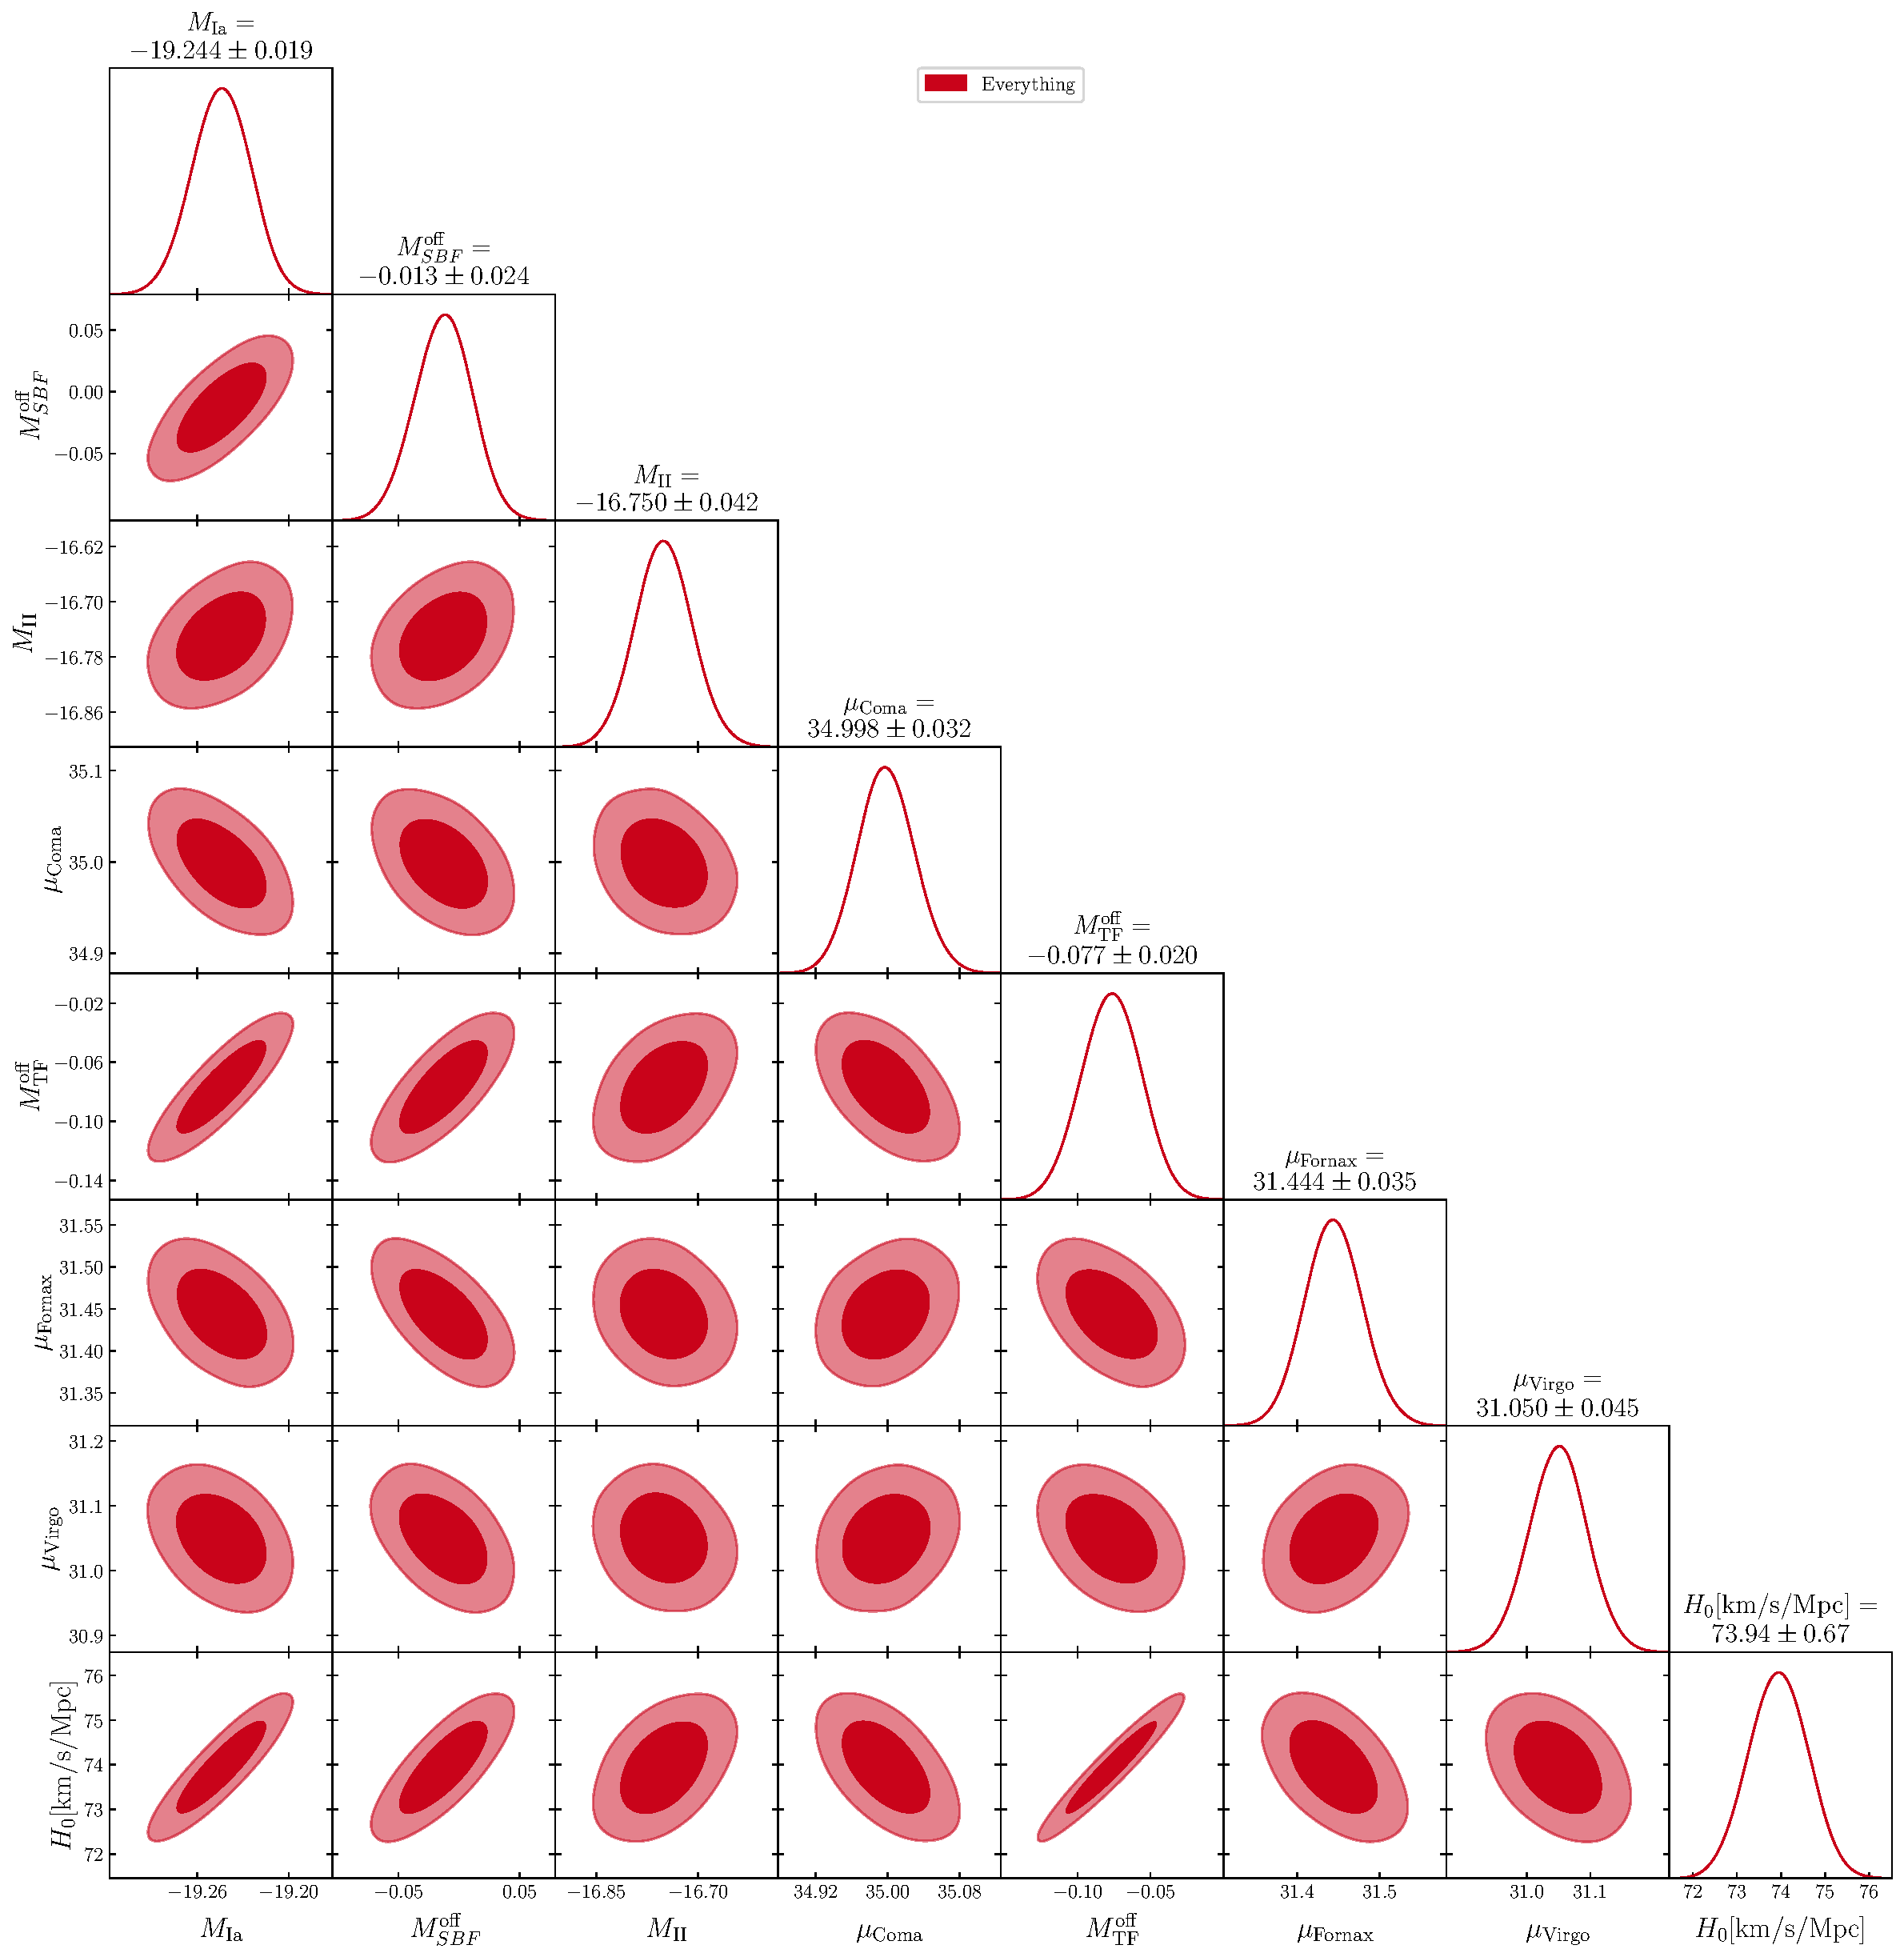
\includegraphics[width=0.9\linewidth]{Figures/chains_all_title_forpub.pdf}
    \caption{Corner plot illustrating the main optimization parameters for the all-inclusive solution, using the naming convention of Appendix~\ref{sec:optimization_parameters}.  Parameters related to individual host distances are not included. Note that this solution is not an alternative result to the baseline solution, but rather a variant to check the impact of further data on our result, see also Section~\ref{sec:variants}. We show it here to highlight the existing correlations between the various (most important) solution parameters. Deviations from the analytically calculated result are due to the numerical precision of a finite-length chain.}
    \label{fig:everything_corner}
\end{figure}

\subsection{Consistency Checks\label{sec:consistency_both}}
We demonstrated the statistical consistency of the baseline solution by building alternate paths through the \DN{} capable of determining \Hcst{}. Statistically independent paths are discussed in Sect.\,\ref{sec:orthogonal_paths}, statistically not independent paths in Sect.\,\ref{sec:consistency_checks}. Replications of \Hcst{} results from the literature are presented in Appendix~\ref{sec:comparisons}.

\subsubsection{Orthogonal paths}\label{sec:orthogonal_paths}

Orthogonal paths strike statistically fully independent paths across the \DN{}. In creating these paths, we sought to identify configurations capable of achieving similar constraining power.
We identified the following two\footnote{In principle, more orthogonal paths could be formulated (e.g., by separating out specific one-step methods), but such combinations of paths are typically not balanced in their constraining power.} orthogonal paths and two extensions of the latter:
\begin{itemize}
    \item \textbf{O1:(MW+LMC+SMC+Ceph+SNIa+FP)} employs the Magellanic Clouds and MW parallaxes as anchors, calibrates SNeIa using Cepheids, and adds in the FP calibrated in Coma. This yields $\Hcst = 73.11 \pm 0.92 \Hunit$ with a $\chi^2=53.5$ and a reduced $\chi^2$ of 0.922.
    \item \textbf{O2:(N4258+TRGB+SBF+MM)} Uses N4258 as anchor, TRGB as calibrators, and SBF as tracers, in addition to megamasers. This corresponds to a modified V07 (baseline+SMC) from which all measurements correlated with O1 have been removed. This yields $\Hcst = 73.45 \pm 1.78 \Hunit$, with a $\chi^2=11.2$, and a reduced  $\chi^2$ of 0.4853. The low reduced $\chi^2$ indicates that the measurement uncertainties used are overestimated.
    \item \textbf{O2\_V99a:(O2+SNII+EPM)} Modified O2 to which both astrophysically and empirically calibrated SNe\,II have been added, i.e., corresponds to V99a without elements in O1. We find $\Hcst = 74.06 \pm 1.25 \Hunit$, with a $\chi^2=28.76$, and a reduced  $\chi^2$ of 0.5752. Here too the reduced $\chi^2$ is a little low.
    \item \textbf{O2\_V99:(O2\_V99a+TF)} Modified O2 with Tully-Fisher relation added, i.e., corresponds to V99 without the elements in O1. We find $\Hcst = 74.93 \pm 1.14 \Hunit$, with a $\chi^2=186.6631$, and a reduced  $\chi^2$ of 1.4359. The very significant increase in reduced $\chi^2$ emphasizes the underestimated uncertainties of the Tully-Fisher results, cf. V99.
\end{itemize} 
Fig.\,\ref{fig:paths_orth} illustrates the results of these orthogonal paths compared to the baseline result. Both O1 and O2 are highly compatible with each other, deviating by only $0.17\sigma$ despite representing fully independent measurements. As previously shown in the context of V13, the significantly higher uncertainty of O2 is due to the exclusion of SNe\,Ia. 
The orthogonal nature of O1 and O2 allows to compute their weighted average, $H_0^\mathrm{O1+O2} = (73.18\pm 0.82)\Hunit$, which agrees to within $0.3\,$\Hunit{} of the baseline. The slightly offset central value and reduced precision arise due to fewer internal cross-calibrations---their combination is missing for example any N4258-anchored calibrations of SNe~Ia. This underlines a key advantage of the covariance-combined approach taken by the H0DN collaboration compared to independent pursuits of \Hcst{}\,.

The two extensions to O2 considered, O2\_V99a and VO2\_V99, add elements from the ``everything'' variants (V99a, V99) to improve precision. Both extensions yield \Hcst{} values marginally higher than O2 and fully compatible with the respective ``everything'' variants V99 and V99a. The weighted average $H_0^\mathrm{O1+O2\_V99a} = (73.45\pm 0.74)\Hunit$ agrees to within $< 0.5\sigma$ with V99a and features a very similar uncertainty. Finally, the weighted average including the Tully-Fisher relation, $H_0^\mathrm{O1+O2\_V99} = (73.77\pm 0.71)\Hunit$, agrees to within $0.4$\,\Hunit{} with V99, with also very similar uncertainty.

Overall these tests confirm both the reliability of the main results as well as the consistent setup of the network. We note that in the case in which the baseline is split into two orthogonal paths we have a mild domination of the uncertainty by the SNe~Ia, whereas in the extended cases the uncertainties are relatively balanced.

\subsubsection{Paths based on subsets of data} \label{sec:consistency_checks}

In order to verify the internal consistency of different data sets and methods relevant to determining the Hubble constant, 
we show below the $H_0$ values obtained for a set of ``paths'' through the network, each defined by a unique combination of anchors, calibrators, and tracers.\footnote{In practice we construct these paths as minimal combinations, except where this might lead to ambiguities. First we use each of the possible calibrator sets (e.g. Cepheids measured with HST, or Miras, or JAGB, etc.) together with the SNe~Ia as Hubble flow tracers (13 combinations), then using the SNe~II (either just with the minimal calibrator set from \citet{2020MNRAS.496.3402D} or with all available calibrators) (2 combinations), the megamasers alone, the SBF anchored using any hosts anchored by NGC$\,$4258, and the SNII tailored~EPM method (each 1 path), as well as the FP method anchored only by the SBF value (to remain minimal). In total that makes 19 paths through the network.} These paths are not all statistically independent by definition, since they might share, for example, a common anchor or a common set of tracer objects. However, we expect the corresponding distribution of $H_0$ values to align at least as well as for independent variables, since we expect the shared data to produce positive, not negative, correlations. In this case, the corresponding test statistics can be regarded as lower bounds on the true values that would be obtained if the full correlation structure were accounted for (i.e., in plain English: ``if the points sharing the same data are incompatible, that's even worse than points not sharing the same data being incompatible''). We find that the Anderson-Darling test \textit{cannot} reject the null hypothesis of the paths stemming from a Gaussian distribution at 5\% confidence level, and we find $p=86.3\%$ for the Shapiro test, both very well within acceptable bounds. We also find no visually strong $(>2\sigma)$ outliers among the paths shown in Figure~\ref{fig:paths_consistency}. Note that since these paths are constructed always using minimal paths through the network, they explicitly do not qualify as `variants' in the sense defined above. We also note that if we were to include the Tully-Fisher case in the generation of these paths, the results worsen quite a bit, to a $p \simeq 10\%$ for the Anderson-Darling test and a $p\simeq 5\%$ for the Shapiro test, showing once again the high discrepancy of the Tully-Fisher based results within the {\DN}.

\begin{figure}
    \centering
    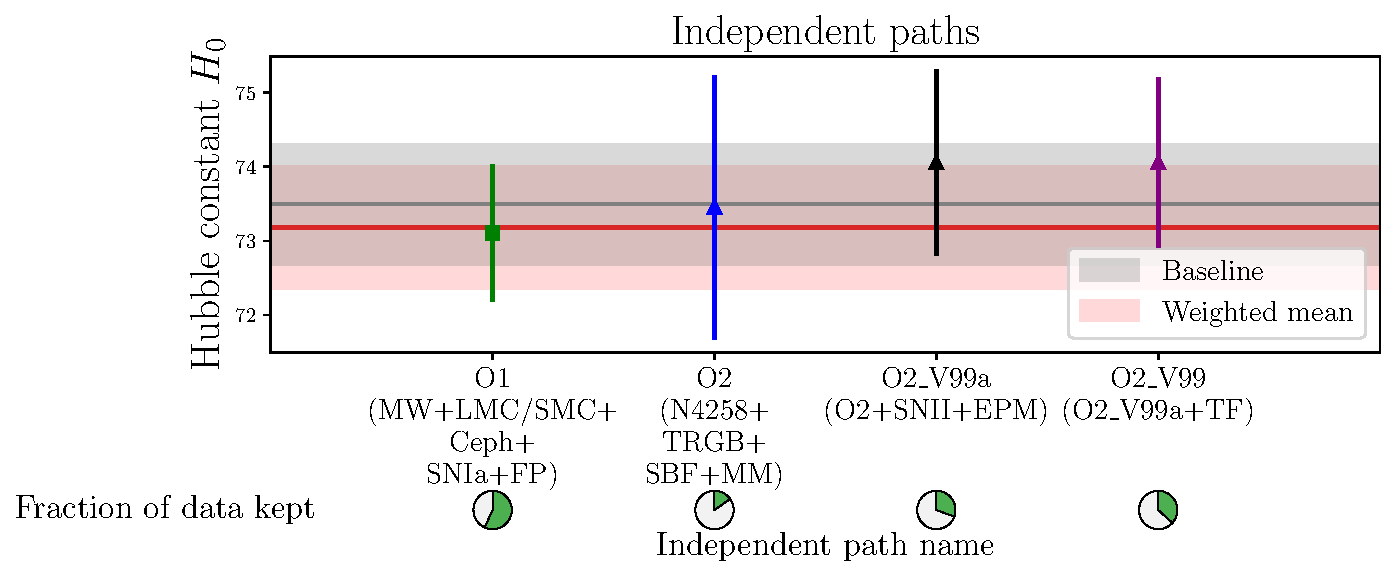
\includegraphics[width=0.79\linewidth]{Figures/o_paths_v3.pdf}
    \caption{The two paths starting with ``O'' are proper orthogonal paths and can be taken as independent measurements of the Hubble constant. Their weighted mean (red) agrees well with our baseline result despite the latter including all cross-correlations. The shortcuts of the data sets are as defined in the text. The pie charts  ``fraction of data kept'' represent the fraction of statistical power remaining in the path. It is computed as the fraction of the variance of {\Hcst} for the given result (in this way multiple datasets with the same constraining power in $H_0$ will be assigned equal percentages). We show the percentages relative to the baseline result (V00).}
    \label{fig:paths_orth}
\end{figure}

\begin{figure}
    \centering
    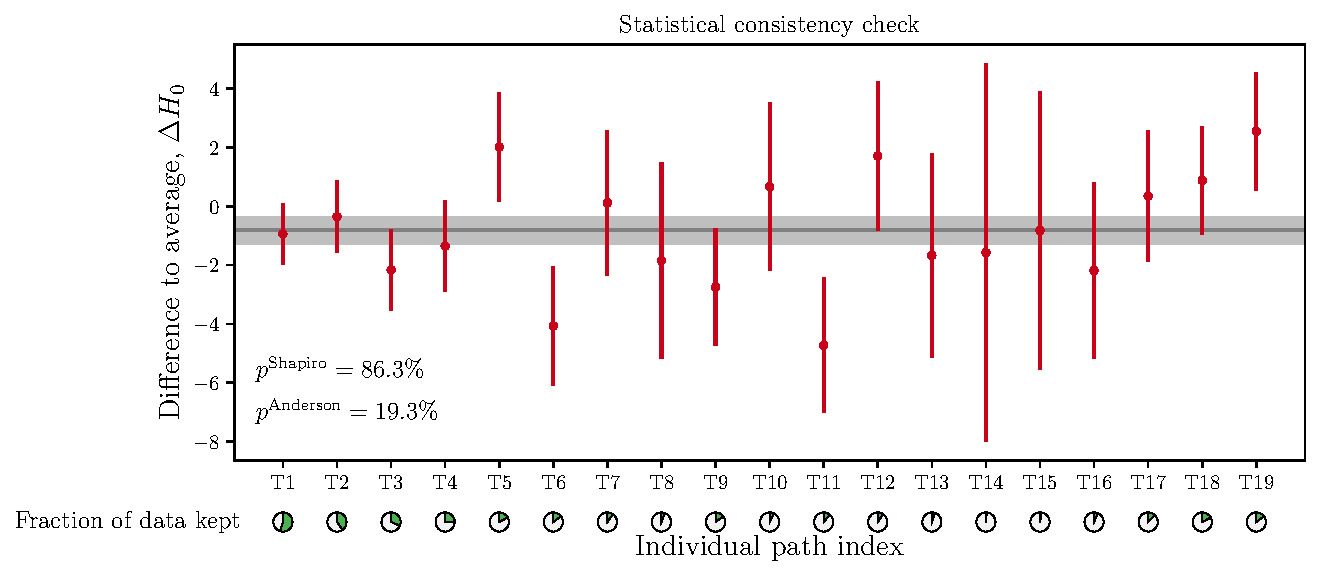
\includegraphics[width=0.79\linewidth]{Figures/paths_v6.pdf} 
    \caption{The statistical consistency of various individual paths through the network. These represent a set of paths that are highly correlated, and often only take a tiny part of the network into account. They are used for a statistical consistency check and should not be interpreted as valid variants in the sense of section \ref{sec:select_variants}. We also show the simple weighted mean of these paths in grey purely for visual purposes, reminding that due to their correlations (and selection effects) it need not necessarily agree with the baseline result. For details on the pie charts, see Fig.~\ref{fig:paths_orth}.}
    \label{fig:paths_consistency}
\end{figure}
